\begin{center}
    \Large\bfseries LAMPIRAN
\end{center}
\vspace{1cm}

% === LAMPIRAN 1 ===
\begin{center}
    % Menampilkan gambar surat terlebih dahulu
    % Tinggi disetel 0.73\textheight agar ruang halaman cukup untuk judul LAMPIRAN di atas dan label di bawah
    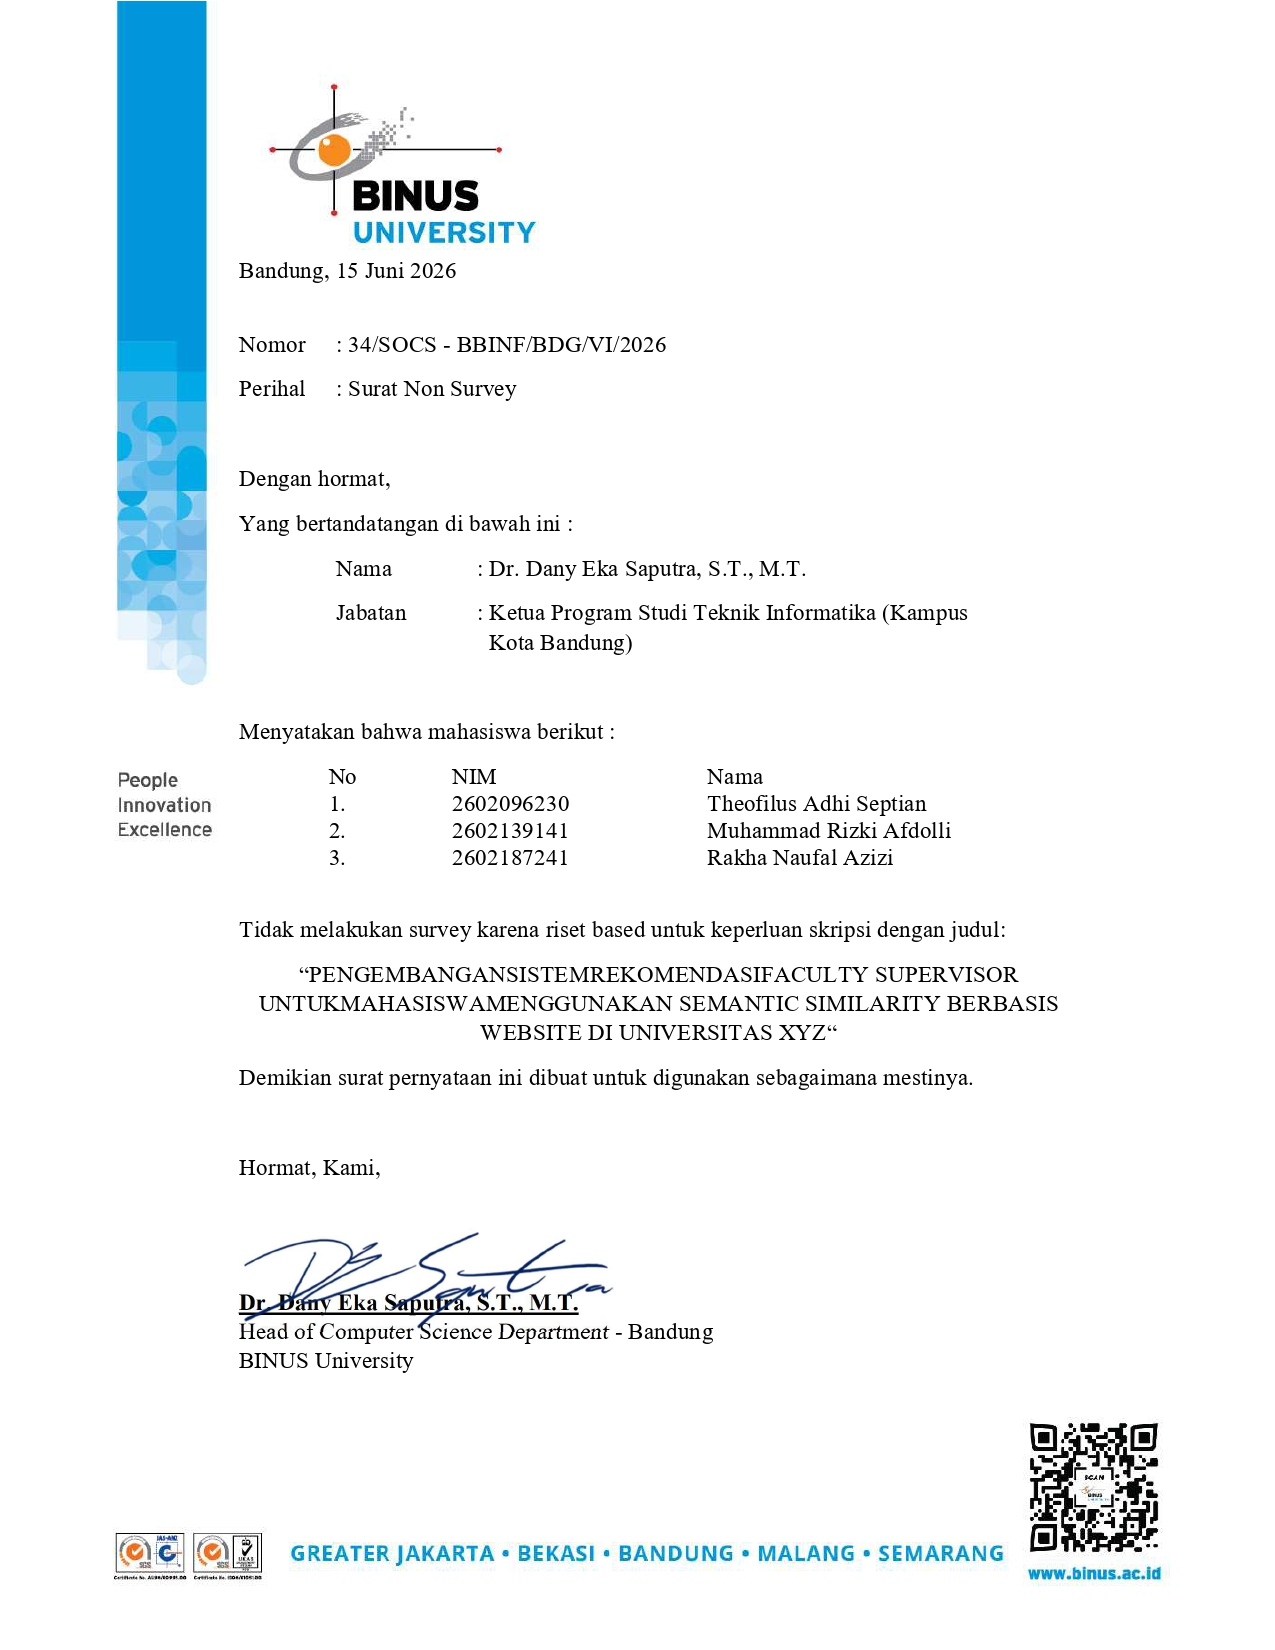
\includegraphics[height=0.73\textheight]{pic/suratsurvey.jpg}
    
    \vspace{0.5cm}
    % Keterangan ditaruh di bawah gambar dengan format miring (italic) sesuai referensi
    \textit{\large Lampiran 1 Surat Survei Mahasiswa}
\end{center}
\newpage

% === LAMPIRAN 2 ===
\noindent\textbf{\large Lampiran 2: Jadwal Kegiatan dan Penelitian}
\vspace{0.4cm}

Berikut adalah jadwal kegiatan penelitian yang dilakukan selama proses pengerjaan skripsi ini, mulai dari bulan September 2025 hingga Juni 2026. [cite: 13, 56, 1653]

\begin{table}[htbp]
\centering
\renewcommand{\thetable}{2.1} % Penomoran otomatis menjadi Tabel 2.1 mengikuti Lampiran 2
\caption{Jadwal Kegiatan Penelitian}
\label{tab:jadwal_kegiatan}
\vspace{0.3cm}

\small 
\setlength{\tabcolsep}{4pt} 

\begin{tabular}{|p{4.8cm}|c|c|c|c|c|c|c|c|c|c|}
\hline
\textbf{Jenis Kegiatan} & \multicolumn{4}{c|}{\textbf{2025}} & \multicolumn{6}{c|}{\textbf{2026}} \\ \cline{2-11} 
 & \textbf{Sep} & \textbf{Okt} & \textbf{Nov} & \textbf{Des} & \textbf{Jan} & \textbf{Feb} & \textbf{Mar} & \textbf{Apr} & \textbf{Mei} & \textbf{Jun} \\ \hline

Studi Literatur dan Tinjauan Pustaka & $\bullet$ & $\bullet$ & & & & & & & & \\ \hline
Analisis Masalah dan Kebutuhan Sistem & & $\bullet$ & $\bullet$ & & & & & & & \\ \hline
Pengumpulan Data Wawancara & & $\bullet$ & & & & & & & & \\ \hline
Penyusunan Bab 1 (Pendahuluan) & & & $\bullet$ & & & & & & & \\ \hline
Penyusunan Bab 2 (Tinjauan Pustaka) & & & $\bullet$ & $\bullet$ & & & & & & \\ \hline
Perancangan Sistem (UML, Arsitektur) & & & $\bullet$ & $\bullet$ & & & & & & \\ \hline
Penyusunan Bab 3 (Metode Penelitian) & & & $\bullet$ & $\bullet$ & & & & & & \\ \hline
Pengembangan Sistem (Implementasi) & & & $\bullet$ & $\bullet$ & $\bullet$ & $\bullet$ & $\bullet$ & $\bullet$ & $\bullet$ & \\ \hline
Pengujian dan Evaluasi Sistem & & & & & & & & $\bullet$ & $\bullet$ & \\ \hline
Penyusunan Bab 4 (Hasil dan Pembahasan) & & & & & & & & $\bullet$ & $\bullet$ & $\bullet$ \\ \hline
Penyusunan Bab 5 (Simpulan dan Saran) & & & & & & & & & $\bullet$ & $\bullet$ \\ \hline
Revisi dan Finalisasi Dokumen & & & & & & & & & & $\bullet$ \\ \hline

\end{tabular}
\end{table}

\newpage

% === LAMPIRAN 3 ===
\noindent\textbf{\large Lampiran 3: Tautan Repository dan Dokumen Pendukung}
\vspace{0.4cm}

Berikut adalah tautan-tautan yang berkaitan dengan penelitian ini, meliputi repositori kode sumber, dokumen skripsi, serta instrumen pengumpulan data. [cite: 1657]
\vspace{0.3cm}

\begin{table}[htbp]
\centering
\renewcommand{\thetable}{3.1} % Penomoran otomatis menjadi Tabel 3.1 mengikuti Lampiran 3
\caption{Daftar Tautan Pendukung Penelitian}
\label{tab:tautan_pendukung}
\vspace{0.3cm}

\small
\begin{tabular}{|c|p{4.5cm}|p{8.5cm}|}
\hline
\textbf{No.} & \textbf{Keterangan} & \textbf{Tautan} \\ \hline

1 & Repository Kode Sumber Sistem Rekomendasi & 
\raggedright \texttt{https://github.com/\allowbreak rizkiafdl/\allowbreak faculty-recommender-thesis} \tabularnewline \hline

2 & Repository Dokumen Skripsi (LaTeX) & 
\raggedright \texttt{https://github.com/\allowbreak rizkiafdl/\allowbreak latex-recomendation-system} \tabularnewline \hline

3 & Google Form Wawancara & 
\raggedright \texttt{https://docs.google.com/\allowbreak forms/d/e/\allowbreak 1FAIpQLSfWDj3e4Xc\allowbreak 2C01WKA1sZ678JEMajcQ\allowbreak 6110aUIOmKWGRgJYQ/\allowbreak viewform?usp=dialog} \tabularnewline \hline

4 & Spreadsheet Hasil Wawancara & 
\raggedright \texttt{https://docs.google.com/\allowbreak spreadsheets/d/\allowbreak 12wOS4fbvfyNWXB5pDLm-\allowbreak ZomiBE5gsTlkulVt\allowbreak U1cvs/edit?usp=sharing} \tabularnewline \hline

\end{tabular}
\end{table}